%
\normalsize%
\subsection{Protocol}%
\label{sec:paml:Protocol}%
A \paml{Protocol} describes how to carry out some form of laboratory or research process.
              For example, a \paml{Protocol} could describe DNA miniprep, Golden-Gate assembly, a cell culture experiment.
              At present this class adds no additional information over \uml{Activity}, but may in the future.%
\newline%
\linebreak%


\begin{figure}[h!]%
\centering%
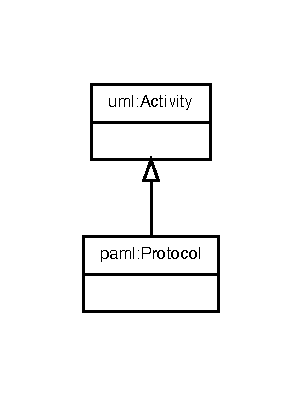
\includegraphics[width=0.21595744680851064\textwidth]{paml_classes/Protocol_abstraction_hierarchy.pdf}%
\caption{Protocol}%
\label{fig:Protocol}%
\end{figure}

%
The \paml{Protocol} class is shown in \ref{fig:Protocol}. It is derived from \uml{Activity}.%
%
\subsection{Primitive}%
\label{sec:paml:Primitive}%
A \paml{Primitive} describes a library function that acts as a basic ``building block'' for a \paml{Protocol}.
              For example, a \paml{Primitive} could describe pipetting, measuring absorbance in a plate reader, or centrifuging.
              At present this class adds no additional information over \uml{Behavior}, but may in the future.%
\newline%
\linebreak%


\begin{figure}[h!]%
\centering%
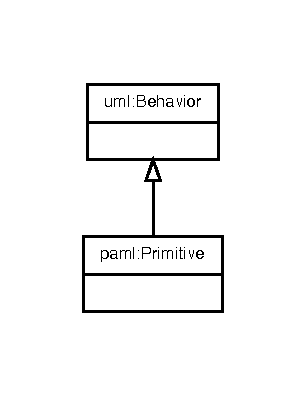
\includegraphics[width=0.21893617021276596\textwidth]{paml_classes/Primitive_abstraction_hierarchy.pdf}%
\caption{Primitive}%
\label{fig:Primitive}%
\end{figure}

%
The \paml{Primitive} class is shown in \ref{fig:Primitive}. It is derived from \uml{Behavior}.%
%
\subsection{BehaviorExecution}%
\label{sec:paml:BehaviorExecution}%
A \paml{BehaviorExecution} is a record of how a \paml{Protocol}, \paml{Primitive}, or other \uml{Behavior} was carried out.
        The execution of the behavior could be either real or simulated.

        In specifying a \paml{BehaviorExecution}, the prov:type field inherited from \prov{Activity} is used to indicate the
        \uml{Behavior} whose execution is being recorded. Precisely \sbol{one} value of prov:type MUST be a URI for a \uml{Behavior}.
        The prov:startedAtTime and prov:endedAtTime fields SHOULD be used to record timing information as this becomes
        available.
        Finally, the entity carrying out the execution SHOULD be recorded as a \prov{Agent} indicated using a
        \prov{Association}.

        Note that a \paml{BehaviorExecution} can be used to record both the state of an in-progress execution as well as an
        execution that has completed. As a \paml{BehaviorExecution} proceeds, all values of its properties are monotonic,
        i.e., they are only added to and never changed.

        TODO: need to changing completedNormally to allow indication of an in-progress BehaviorExecution
        TODO: Is there a good ontology for agent roles in association?%
\newline%
\linebreak%


\begin{figure}[h!]%
\centering%
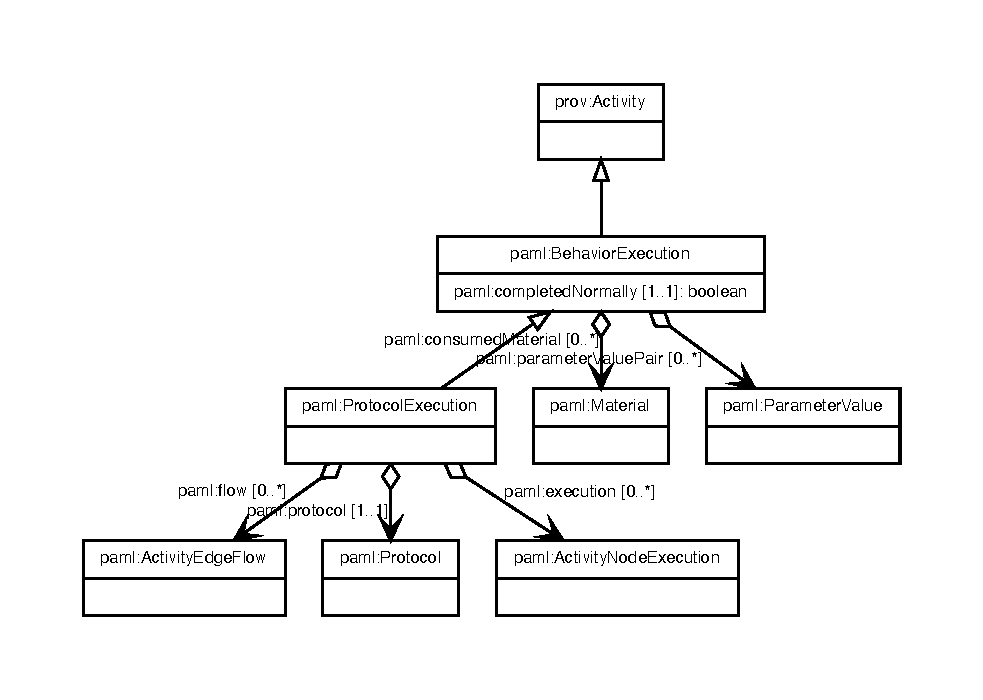
\includegraphics[width=0.7327659574468085\textwidth]{paml_classes/BehaviorExecution_abstraction_hierarchy.pdf}%
\caption{BehaviorExecution}%
\label{fig:BehaviorExecution}%
\end{figure}

%
The \paml{BehaviorExecution} class is shown in \ref{fig:BehaviorExecution}. It is derived from \prov{Activity} and includes the following specializations: \paml{ProtocolExecution}. %
This class includes the following properties: \paml{completedNormally}, \paml{parameterValuePair}, \paml{consumedMaterial}. %
\begin{itemize}%
\item%
The \paml{parameterValuePair} property is OPTIONAL and contains URI references to associated objects of type ParameterValueThe parameterValuePair property is used to record the value that was associated with each
        uml:Parameter for the uml:Behavior when it was executed, by means of a ParameterValue object.
        Any uml:Parameter that is not listed is assumed to have had no value assigned. Conversely, every non-optional
        uml:Parameter for the uml:Behavior MUST have an associated parameter value.
        Finally, note that this applies both to input uml:Parameter objects, whose value is set before execution begins,
        and to output uml:Parameter objects, whose value is set by the time execution ends.

        TODO: are multiple values allowed, or do those need to be passed as list/set types?
        %
\item%
The \paml{consumedMaterial} property is OPTIONAL and contains URI references to associated objects of type MaterialThis property is used to record the noteworthy consumables used during the execution of the
        Behavior. For example, a cell culture protocols will consume various reagents and samples of cells. Materials
        with the same specification SHOULD be consolidated, such that the list of materials SHOULD NOT contain two
        materials with the same specification.

        For example, consuming 5.0 mL of PBS and 2.0 mL of PBS should be recorded as consuming 7.0 mL of PBS.
        Complex materials, however, MAY contain the same material more than once in their substructure.
        For example, M9 media contains glucose, but it would not be necessary to consolidate the glucose in M9 media
        with additional glucose that was added as a supplement, since that would change the definition of the media.%
\item%
The \paml{completedNormally} property is REQUIRED and has a singleton value of type booleanThis boolean should be set to true if the Behavior completed normally and false if there
        was some exception condition. At present, no further information is being encoded about exceptions, but this
        is an extension that is anticipated for the future.%
\end{itemize}%
\subsubsection{ProtocolExecution}%
\label{sec:paml:ProtocolExecution}%
A \paml{ProtocolExecution} expands on the information in a \paml{BehaviorExecution} by including records for
        the nodes and edges defining the Protocol's behavior as a \uml{Activity}. Specifically, the execution property
        is used to record each firing of a \uml{ActivityNode} and the flow property is used to record each time a token
        moves along a \uml{ActivityEdge}.
        Otherwise, a \paml{ProtocolExecution} is used exactly the same way as its parent class \paml{BehaviorExecution}.

        TODO: consider dropping the protocol field as redundant with use prov:type field in its parent%
\newline%
\linebreak%
The \paml{ProtocolExecution} class is shown in \ref{fig:BehaviorExecution}. It is derived from \paml{BehaviorExecution}.%
This class includes the following properties: \paml{execution}, \paml{protocol}, \paml{flow}. %
\begin{itemize}%
\item%
The \paml{execution} property is OPTIONAL and contains URI references to associated objects of type ActivityNodeExecutionEach instance of this property links to an ActivityNodeExecution that records one
        firing of a uml:ActivityNode during the execution of its containing Protocol%
\item%
The \paml{protocol} property is REQUIRED and contains a URI reference to an associated object of type ProtocolThis property appears to be redundant with the use of prov:type specified by BehaviorExecution, and is likely to be deleted%
\item%
The \paml{flow} property is OPTIONAL and contains URI references to associated objects of type ActivityEdgeFlowEach instance of this property links to an ActivityEdgeFlow that records one movement of a UML
        token along a uml:ActivityEdge during the execution of its containing Protocol%
\end{itemize}%
\subsection{ParameterValue}%
\label{sec:paml:ParameterValue}%
This class is used to represent the assignment of a value to a parameter in a BehaviorExecution
        that records the execution of a \uml{Behavior}. This class is similar to \prov{Usage}, but instead of always
        pointing to an object it uses an arbitrary literal (which might or might not be an object). An example would
        be recording that a plate reader absorbance measurement was taken with its absorbance wavelength parameter set
        to 600 nm%
\newline%
\linebreak%


\begin{figure}[h!]%
\centering%
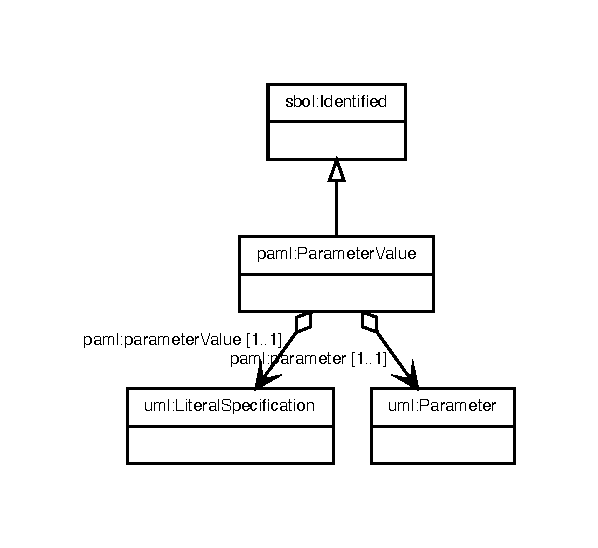
\includegraphics[width=0.42148936170212764\textwidth]{paml_classes/ParameterValue_abstraction_hierarchy.pdf}%
\caption{ParameterValue}%
\label{fig:ParameterValue}%
\end{figure}

%
The \paml{ParameterValue} class is shown in \ref{fig:ParameterValue}. It is derived from \sbol{Identified}.%
This class includes the following properties: \paml{parameter}, \paml{parameterValue}. %
\begin{itemize}%
\item%
The \paml{parameter} property is REQUIRED and contains a URI reference to an associated object of type ParameterThis property points to the uml:Parameter associated with the value (e.g., wavelength for a
        plate reader absorbance measurement behavior).%
\item%
The \paml{parameterValue} property is REQUIRED and contains a URI reference to an associated object of type LiteralSpecificationThis property points to the literal value used for the parameter during execution (e.g., a
        uml:LiteralIdentified for an om:Measure representing a 600 nm wavelength).%
\end{itemize}%
\subsection{Material}%
\label{sec:paml:Material}%
An amount of material allocated for use during the execution of a behavior.
        For example a \paml{Material} might be used to specify 1 96-well flat-bottom microplate or 2.5 mL of 10 millimolar glucose.

        TODO: consider changing type of specification to allow non-TopLevel descriptions, such as a \paml{ContainerSpec} or sbol:ExternallyDefined
        TODO: consider adding a field to distinguish between expended vs. reusable materials.%
\newline%
\linebreak%


\begin{figure}[h!]%
\centering%
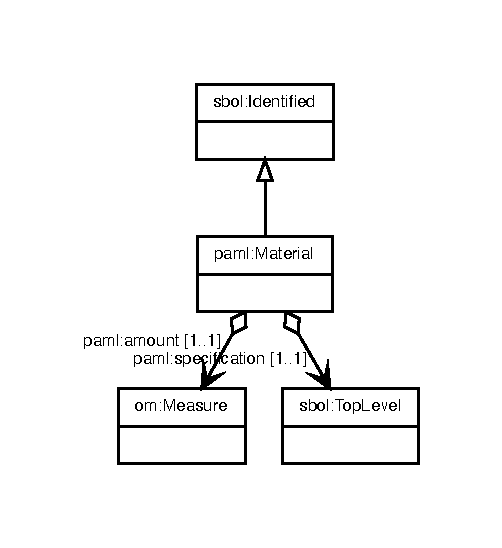
\includegraphics[width=0.35893617021276597\textwidth]{paml_classes/Material_abstraction_hierarchy.pdf}%
\caption{Material}%
\label{fig:Material}%
\end{figure}

%
The \paml{Material} class is shown in \ref{fig:Material}. It is derived from \sbol{Identified}.%
This class includes the following properties: \paml{amount}, \paml{specification}. %
\begin{itemize}%
\item%
The \paml{amount} property is REQUIRED and contains a URI reference to an associated object of type MeasureThe amount property of a Material is used to indicate the quantity of material used.
        For example, 2.5 mL (referring to a fluid) or 3 (with unit "number", referring to a group of microplates)%
\item%
The \paml{specification} property is REQUIRED and contains a URI reference to an associated object of type TopLevelThe specification property is used to indicate the type of material used.
        For example a DNA sample would be described by an sbol:Component.

        TODO: add example for glucose and for 96-well plate%
\end{itemize}%
\subsection{ActivityEdgeFlow}%
\label{sec:paml:ActivityEdgeFlow}%
An \paml{ActivityEdgeFlow} records \sbol{one} movement of a UML token along a \uml{ActivityEdge} during the
        execution of its containing \paml{Protocol}. If the edge is a \uml{ObjectFlow}, then the value MUST be set.
        If the edge is a \uml{ControlFlow}, then the value MUST NOT be set.

        For instance, the \paml{ActivityEdgeFlow} for a \uml{ObjectFlow} might record a measurement being sent to an output
        \uml{Parameter}, while the \paml{ActivityEdgeFlow} for a \uml{ControlFlow} might record a decision to proceed down a
        particular branch from a \uml{DecisionNode}.

        Note that a \uml{ActivityEdge} might appear in multiple \paml{ActivityEdgeFlow} records associated with a single
        \paml{ProtocolExecution}, e.g., due to a loop in the \paml{Protocol}.  It also might not appear in any, if the
        \uml{ActivityEdge} is on a path not taken due to branching control flow.

        TODO: correct the cardinality: edgeValue is supposed to be optional, not edge
        %
\newline%
\linebreak%


\begin{figure}[h!]%
\centering%
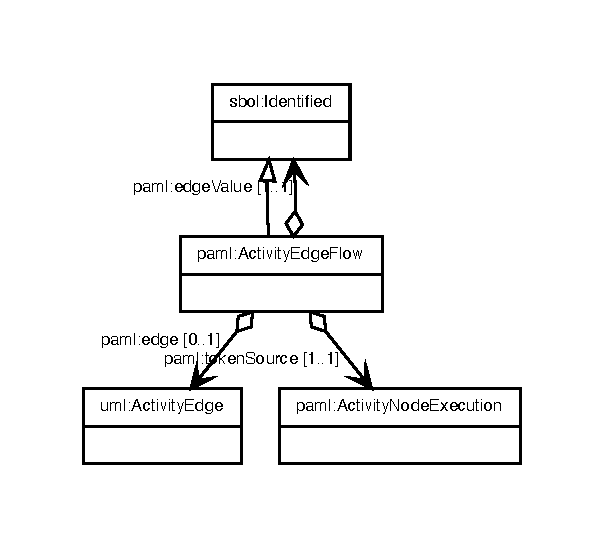
\includegraphics[width=0.4319148936170213\textwidth]{paml_classes/ActivityEdgeFlow_abstraction_hierarchy.pdf}%
\caption{ActivityEdgeFlow}%
\label{fig:ActivityEdgeFlow}%
\end{figure}

%
The \paml{ActivityEdgeFlow} class is shown in \ref{fig:ActivityEdgeFlow}. It is derived from \sbol{Identified}.%
This class includes the following properties: \paml{tokenSource}, \paml{edge}, \paml{edgeValue}. %
\begin{itemize}%
\item%
The \paml{tokenSource} property is REQUIRED and contains a URI reference to an associated object of type ActivityNodeExecutionThis property is used to indicate the ActivityNodeExecution that produced the token.%
\item%
The \paml{edge} property is OPTIONAL and contains a URI reference to an associated object of type ActivityEdgeThis property is used to indicate the uml:ActivityEdge down which the token moved.%
\item%
The \paml{edgeValue} property is REQUIRED and contains a URI reference to an associated object of type IdentifiedThis property is used to indicate the value of a token that moved on a uml:ObjectFlow edge.%
\end{itemize}%
\subsection{ActivityNodeExecution}%
\label{sec:paml:ActivityNodeExecution}%
An \paml{ActivityNodeExecution} records \sbol{one} instance in which a \uml{ActivityNode} is executed during the
        execution of its containing \paml{Protocol}.

        For instance, the \paml{ActivityNodeExecution} for a \uml{CallBehaviorAction} to measure absorbance on a plate reader
        would set its node property to point to the \uml{CallBehaviorAction} and might have incomingFlow properties
        indicating arrival of information about the samples to measure via a \uml{ObjectFlow} and the arrival a
        of permission to begin via a \uml{ControlFlow}.

        Note that a \uml{ActivityNode} might appear in multiple \paml{ActivityNodeExecution} records associated with a single
        \paml{ProtocolExecution}, e.g., due to a loop in the \paml{Protocol}.  It also might not appear in any, if the
        \uml{ActivityNode} is on a path not taken due to branching control flow.%
\newline%
\linebreak%


\begin{figure}[h!]%
\centering%
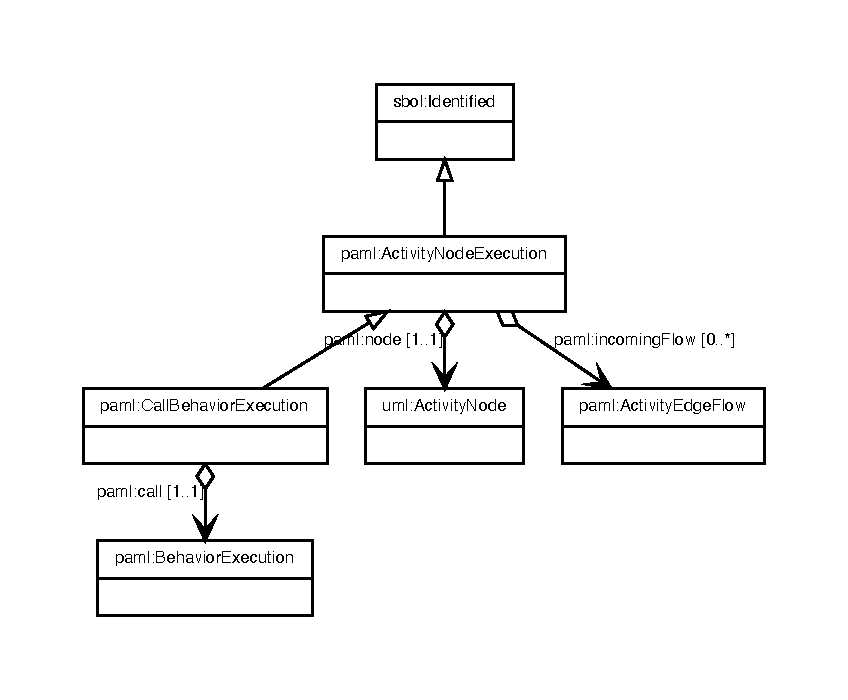
\includegraphics[width=0.6061702127659574\textwidth]{paml_classes/ActivityNodeExecution_abstraction_hierarchy.pdf}%
\caption{ActivityNodeExecution}%
\label{fig:ActivityNodeExecution}%
\end{figure}

%
The \paml{ActivityNodeExecution} class is shown in \ref{fig:ActivityNodeExecution}. It is derived from \sbol{Identified} and includes the following specializations: \paml{CallBehaviorExecution}. %
This class includes the following properties: \paml{node}, \paml{incomingFlow}. %
\begin{itemize}%
\item%
The \paml{node} property is REQUIRED and contains a URI reference to an associated object of type ActivityNodeThis property is used to indicate the uml:ActivityNode that has been execcuted.%
\item%
The \paml{incomingFlow} property is OPTIONAL and contains URI references to associated objects of type ActivityEdgeFlowThis property is used to indicate an ActivityEdgeFlow that delivered a token consumed during
        the execution of the uml:ActivityNode.%
\end{itemize}%
\subsubsection{CallBehaviorExecution}%
\label{sec:paml:CallBehaviorExecution}%
A \paml{CallBehaviorExecution} extends \paml{ActivityNodeExecution} by adding a pointer to a BehaviorExecution
        record for the \uml{Behavior} that is being executed.

        For a primitive action (e.g., measuring absorbance on a plate reader), this is a plain \paml{BehaviorExecution},
        while for calling a \paml{Protocol} as a sub-routine (e.g., to run a stage of an Type IIS assembly), this would be a
        \paml{ProtocolExecution}.%
\newline%
\linebreak%
The \paml{CallBehaviorExecution} class is shown in \ref{fig:ActivityNodeExecution}. It is derived from \paml{ActivityNodeExecution}.%
This class includes the following properties: \paml{call}. %
\begin{itemize}%
\item%
The \paml{call} property is REQUIRED and contains a URI reference to an associated object of type BehaviorExecutionThis property indicates the BehaviorExecution record for the uml:Behavior that was called.%
\end{itemize}%
\subsection{SampleCollection}%
\label{sec:paml:SampleCollection}%
SampleCollection is the base class for describing the collections of physical materials that are
         acted upon by a \paml{Protocol}. For example, a \paml{SampleCollection} might describe a set of 10 cell cultures growing in
         96-well plate cells, or a set of 6 streaked agar plates, or a single 500 mL flask filled with media.

         There are two types of \paml{SampleCollection}. A \paml{SampleArray} specifies an n-dimensional rectangular array of samples,
         all stored in the same type of container. A \paml{SampleMask} specifies a subset of a \paml{SampleCollection} by means of an
         array of Boolean values indicating whether each element is included or excluded from the subset.

         Note, however, that a \paml{SampleCollection} is a logical object and not a physical object. Thus, while a
         \paml{SampleCollection} might describe a set of samples in 96-well plate wells, it does not necessarily identify
         a particular 96-well plate or the location of those wells.  In practice, these will be determined as a
         result of the specific library calls made to generate \paml{SampleCollection} objects, and may not be determined
         until the protocol is actually run in a particular execution environment.

         This is important for increasing the flexibility with which a \paml{Protocol} can be specified and applied.
         Consider, for example, a cell culturing protocol that includes a step to measure \sbol{sample} absorbance on a plate
         reader. Describing this step does not require knowing how the samples are laid out on the plate, and in many
         cases is even acceptable to run on samples across multiple plates. This flexibility will allow the cell
         culturing protocol to be applied for experiments with different numbers and arrangements of samples.%
\newline%
\linebreak%


\begin{figure}[h!]%
\centering%
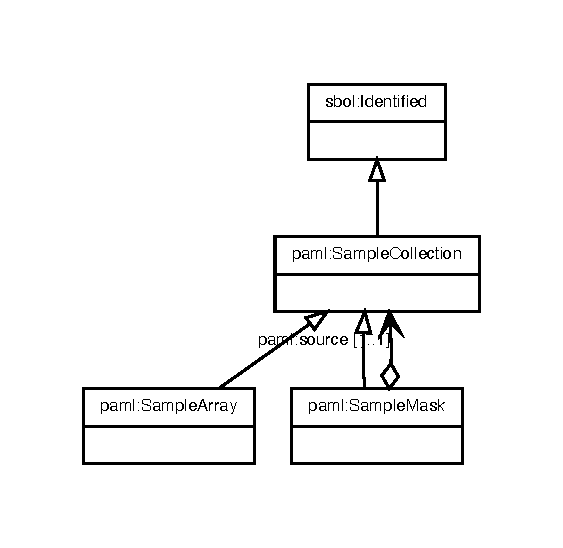
\includegraphics[width=0.40212765957446805\textwidth]{paml_classes/SampleCollection_abstraction_hierarchy.pdf}%
\caption{SampleCollection}%
\label{fig:SampleCollection}%
\end{figure}

%
The \paml{SampleCollection} class is shown in \ref{fig:SampleCollection}. It is derived from \sbol{Identified} and includes the following specializations: \paml{SampleArray}, \paml{SampleMask}. %
%
\subsubsection{SampleArray}%
\label{sec:paml:SampleArray}%
A \paml{SampleArray} specifies an n-dimensional rectangular array of samples, all stored in the same
        type of container. For example, a \paml{SampleCollection} might describe a set of 10 cell cultures growing in
        96-well plate cells, or a set of 6 streaked agar plates, or a single 500 mL flask filled with media.

        Wells may be full, in which case the contents property should contain a URI to a description of the \sbol{sample},
        or empty, in which case the contents should be null.

        Note that this is a logical array, and does not necessarily indicate the actual layout of the samples in space.
        For example, a 2x4 array of samples in 96-well plate wells might end up being laid out as a 2x4 array in wells
        A1 to B4 or as a 2x4 array in wells G5 to H8 or as an 8x1 column in wells A1 to H1, or even as eight wells
        scattered arbitrarily around the plate according to an anti-bias quality control schema.

        This also allows for higher-dimensional arrays where each dimension represents an experimental factor.
        For example, an experiment testing four factors with 3, 3, 4, and 5 values per factor, for a total of 180
        combinations, could be represented as a 4-dimensional \sbol{sample} array of 96-well plate wells, and then end up
        laid out over two plates.

        TODO: need to decide on the format of the contents description.%
\newline%
\linebreak%
The \paml{SampleArray} class is shown in \ref{fig:SampleCollection}. It is derived from \paml{SampleCollection}.%
This class includes the following properties: \paml{contents}, \paml{containerType}. %
\begin{itemize}%
\item%
The \paml{contents} property is REQUIRED and has a singleton value of type stringDescription of the contents.
        TODO: need to decide whether this is a multi-valued property with associated array coordinates or a
        single-valued property with an array value.
        Currently set to string as a "dummy" value that can serialize anything.%
\item%
The \paml{containerType} property is REQUIRED and has a singleton value of type URI%
\end{itemize}%
\subsubsection{SampleMask}%
\label{sec:paml:SampleMask}%
A \paml{SampleMask} is a subset of a \paml{SampleCollection}. The subset of samples to be included is defined
        by an array of Boolean values, where true values indicate that a \sbol{sample} is included and false values indicate
        that it is excluded.

        The dimensions of the mask MUST be identical to the dimensions of the source \paml{SampleCollection}. For this purpose,
        the dimensions of a masked subset are not reduced, but remain the same as the original \paml{SampleArray}. This allows
        masks to be composed, such that SampleMask(source=SampleMask(source=X,mask=mask1),mask=mask2) is equivalent to
        SampleMask(source=X,mask=mask1 AND mask2). Note that this implies masks are commutative and idempotent.%
\newline%
\linebreak%
The \paml{SampleMask} class is shown in \ref{fig:SampleCollection}. It is derived from \paml{SampleCollection}.%
This class includes the following properties: \paml{mask}, \paml{source}. %
\begin{itemize}%
\item%
The \paml{source} property is REQUIRED and contains a URI reference to an associated object of type SampleCollectionThe source indicates the SampleCollection that is being subsetted via the mask%
\item%
The \paml{mask} property is REQUIRED and has a singleton value of type stringThe mask is an N-dimensional array of Booleans values, where each Boolean indicates whether the
        sample at the corresponding location in the source is included in the subset.

        TODO: format of mask array needs to match the array format chosen for the SampleArray contents property%
\end{itemize}%
\subsection{SampleData}%
\label{sec:paml:SampleData}%
The \paml{SampleData} class is used to associate a set of data with a collection of samples.
        This is typically used to capture measurements, e.g., an array of absorbance measurements collected by
        a plate reader. Using this data structure allows the values in a dataframe to be automatically linked to
        the descriptions of the samples that the data describes, which is critical for data analysis.

        The dimensions of the sampleDataValues MUST equal the dimensions of the \paml{SampleCollection} linked with fromSamples.

        TODO: the format of the data values needs to be compatible with the array format chosen for the
        \paml{SampleArray} contents property. In this case, however, we also need to consider how we want to support
        multiple values for each \sbol{sample} (e.g., measurement of both fluorescence and absorbance in a plate reader),
        as well as links to more complex data (e.g., results of flow cytometry or omics for each sample)%
\newline%
\linebreak%


\begin{figure}[h!]%
\centering%
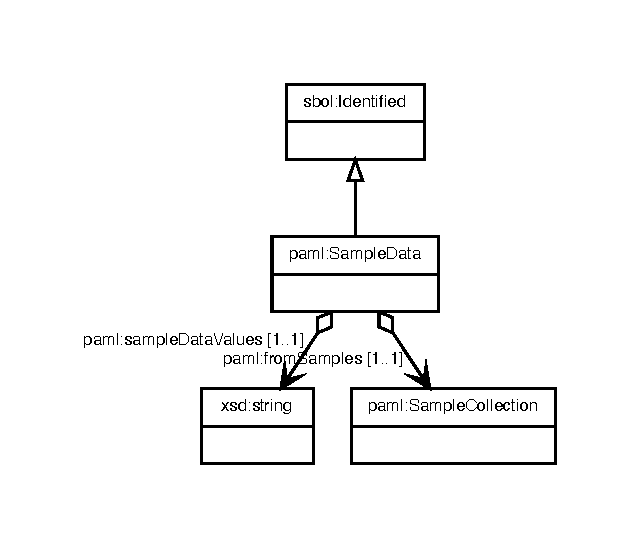
\includegraphics[width=0.3946808510638298\textwidth]{paml_classes/SampleData_abstraction_hierarchy.pdf}%
\caption{SampleData}%
\label{fig:SampleData}%
\end{figure}

%
The \paml{SampleData} class is shown in \ref{fig:SampleData}. It is derived from \sbol{Identified}.%
This class includes the following properties: \paml{fromSamples}, \paml{sampleDataValues}. %
\begin{itemize}%
\item%
The \paml{fromSamples} property is REQUIRED and contains a URI reference to an associated object of type SampleCollectionThe fromSamples property indicates the SampleCollection from which the data were collected.%
\item%
The \paml{sampleDataValues} property is REQUIRED and contains a URI reference to an associated object of type stringThe sampleDataValues are an array of data values, one for each sample, format to be determined.%
\end{itemize}%
\subsection{ContainerSpec}%
\label{sec:paml:ContainerSpec}%
A \paml{ContainerSpec} is used to indicate the type of container to be used for a \paml{SampleArray}, e.g.,
        a standard 96-well flat-bottom transparent plate.

        TODO: determine if we want to use this format or modify it in some way.%
\newline%
\linebreak%


\begin{figure}[h!]%
\centering%
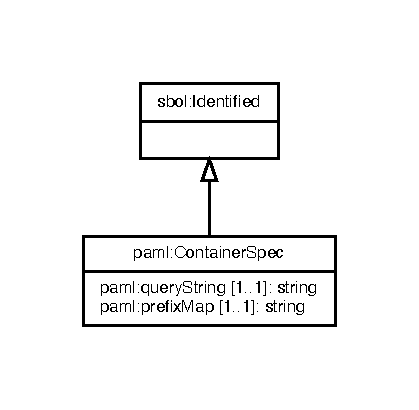
\includegraphics[width=0.29936170212765956\textwidth]{paml_classes/ContainerSpec_abstraction_hierarchy.pdf}%
\caption{ContainerSpec}%
\label{fig:ContainerSpec}%
\end{figure}

%
The \paml{ContainerSpec} class is shown in \ref{fig:ContainerSpec}. It is derived from \sbol{Identified}.%
This class includes the following properties: \paml{prefixMap}, \paml{queryString}. %
\begin{itemize}%
\item%
The \paml{prefixMap} property is REQUIRED and has a singleton value of type stringA prefix map in JSON-LD format, to be applied to a queryString.%
\item%
The \paml{queryString} property is REQUIRED and has a singleton value of type stringA query string, in OWL Manchester syntax, to be used to find matching containers in the ContainerSpec.%
\end{itemize}%
